% !TEX encoding = UTF-8 Unicode
\documentclass[12pt,a4paper,english
% ,twoside,openright
]{tunithesis}

\special{papersize=210mm,297mm}

\author{Roosa Kuusivaara \& Väinö-Waltteri Granat}
\title{Characterizing holographic displays via
numerical simulations - Report} % primary title (for front page)
\thesistype{Laboratory Report} % or Bachelor of Science, Laboratory Report...

\usepackage{lastpage}
\usepackage[english]{babel}
\usepackage[
backend=biber,
style=authoryear,
citestyle=authoryear,
autocite=inline
]{biblatex}
\usepackage{csquotes}
\usepackage{mathrsfs, amsmath}

\addbibresource{references.bib} %Imports bibliography file


\definecolor{tunipurple}{RGB}{78, 0, 142}

\newcommand\todo[1]{{\color{red}!!!TODO: #1}} % Remark text in braces appears in red
\newcommand{\angs}{\textsl{\AA}}              % , e.g. slanted symbol for Ångstöm
% Preparatory content ends here


\pagenumbering{roman} % was: {Roman}
\pagestyle{headings}
\begin{document}

% Special trick so that internal macros (denoted with @ in their name)
% can be used outside the cls file (e.g. \@author)
\makeatletter

% Create the title page.
% First the logo. Check its language.
\thispagestyle{empty}
\vspace*{-.5cm}\noindent

\begin{figure}
    \vspace{-1.3cm}
    \advance\leftskip-2.5cm
    \noindent
\includegraphics{img/tunilogo.png}
\end{figure}
 
\vspace{2.5cm}
\begin{flushright}
\noindent\textsf{\LARGE{\@author}}

\noindent\vspace{0.5cm}

\noindent\Huge{\textsf{\textbf{\textcolor{tunipurple}{\@title}}}}
\end{flushright}
\vspace{13.7cm} % adjust to 12.7 this if thesis title needs two lines

% Last some additional info to the bottom-right corner
\begin{flushright}  
    \begin{spacing}{1.0}
      \textsf{Faculty of Information Technology and Communication Sciences (ITC)\\
      \@thesistype\\
      September 2023}
    \end{spacing}
\end{flushright}

% Leave the backside of title page empty in twoside mode
\if@twoside
\clearpage
\fi

% Turn off page numbering for the first pages
\pagenumbering{gobble}


% Some fields in abstract are automated, namely those with \@ (author,
% title, thesis type).
\chapter*{Abstract}
\begin{spacing}{1.0}
\noindent \@author: \@title\\
\@thesistype\\
Tampere University\\
Master’s Degree Programme in Signal Processing\\
September 2023
\end{spacing}
\noindent\rule{12cm}{0.4pt}

\vspace{0.5cm}

% ---------------------------------------
% Abstract and keywords
% ---------------------------------------

\noindent The abstract is a concise 1-page description of the work: what was the
problem, what was done, and what are the results. Do not include
charts or tables in the abstract.

These instructions are intended for students of Computer Sciences at the Tampere University. They cover questions of writing a thesis, such as use of the literature, structure of the thesis and style, the external appearance of the thesis and the use of tools.  These instructions do not cover the scientific content of the thesis.

~

\noindent\textbf{Keywords:} M.Sc. thesis, layout, writing style.

~


% Add the table of contents


\setcounter{tocdepth}{3}              % How many header level are included
\tableofcontents                      % Create TOC


% The actual text begins here and page numbering changes to 1,2...
% Leave the backside of title empty in twoside mode
\if@twoside
%\newpage
\cleardoublepage
\fi


\renewcommand{\chaptername}{} % This disables the prefix 'Chapter' or
                              % 'Luku' in page headers (in 'twoside'
                              % mode)


\chapter{Introduction}
\label{ch:intro}
\pagenumbering{arabic}
\setcounter{page}{1} 
In this report we describe our work with the `Characterizing holographic displays via
numerical simulations` exercise, for the Advanced Signal Processing Laboratory Course.

In this project we familiarized ourselves with the basics of holographic display, by implementing a part of a holograpics display viewing simulation. We implemented two holographic synthesis methods and a retinal image formation model, by contributing code to a MATLAB codebase given by the course faculty.

\section{Hologram synthesis}
Hologram synthesis describes the method for forming holographic images in 3d space from a given image. In this assignment, instead of using entire 3d space, the analysis can be simplified by considering only a cross section of the 3d space. The hologram is now represented as a 1D array of complex values. This simplification eases the computational load and also makes the process easier to handle.

\section{Retinal Image Formation}

\chapter{Methodology}
\label{sec:methodology}

\section{Implementing Hologram Synthesis}
Our implementation of the holographic image viewer included three different methods of holographic image synthesis, one of which was provided in the code base given to us. The ready made synthesis method was holographic stereograph synthesis (HSS), [TODO: explain hss here]. The first synthesis method we implemented was a Fresnel hologram synthesis which is based on the Fresnel diffraction kernel. The second method we implemented was Rayleigh-Sommerfeld synthesis (RSS), which uses Rayleigh-Sommerfeld diffraction kernel. This formula is similar to the Fresnel but has some differences in calculating the hologram.

\section{Retinal Image Formation Simulation}
To be able to view the synthezised holograms, we had to simulate the viewing process of an eye. This was achieved with a simplified wave propagation model, where human eye is represented by a simple lens and a one-dimensional sensor behind the lens in relation to the viewed hologram.

The transmittance of the lens is described by function~\ref{eq:lens}

\begin{align}
  \label{eq:lens}
  T(s) = exp(\frac{-i\pi}{\lambda f}s^2)
\end{align}

where, $f$ is the focal lenght of the lens.

The propagation of light from the hologram is modeled with a following field function~\ref{eq:field}

\begin{align}
  \label{eq:field}
  U(x;z) = \int \mathscr{F} \{U (\xi;z_0) \} (f_\xi) exp[-2 \pi i (f_\xi x + f_z z)] d f_\xi
\end{align}

where,

\begin{align}
  \label{eq:focus}
  f_z = \sqrt{\frac{1}{\lambda^2} - f_\xi ^ 2}
\end{align}

[TODO: Explain these functions]

The simplified eye model differs from a real human eye in multiple cases. Firstly, sensor of the human eye consists, [TODO: Add stuff]

\subsection{Field propagation implementation}
The implementation of the field progation was provided to us in the code base, in the $propagateField\_PWD.m$ file. The file starts with defining the basic parameters, which are current location of the eye, distance from lens to sensor, the focal length of the eye and the physical size of the hologram plane.

In the next step the file sets up the more complex parts of the simulation, like size of the sensor, properties of the propagating light and the sampling grid.

Finally the file executes the field propagation simulation, where each of the sections of the synthezied hologram are propagated trough the wave field and the results are of the sensor are sampled to produces an image as PSF which is returned from the function.


\chapter{Results}
\label{sec:results}
In this section we anaylze the images produced by the implemented model.

From the simulation we attained an image consisting of multiple overlayed PSF images depicting the hologram formed on the simulated sensor. From the image~\ref{fig:psf_multiple_fresnel} we can see that from the samples the $z_f$ value of $-0.42$ produces the sharpest image, since most of the points fall in the origin. This is different from what would be expected, since in ideal situation the sharpest images should form with the same values as the distance to point source, which in our simulation is $-0.4$. When the value of $z_f$ moves away from $-0.42$ we expected the graph to widen, since image formed won't be as sharp and this is reflected in the figure, as the values closer to $-0.42$ produce higher graphs.

We also repeated this for Rayleigh-Sommerfield synthesis and Holographic stereogram synthesis, as shown in figures~\ref{fig:psf_multiple_rs} and~\ref{fig:psf_multiple_hs}. The result for the Rayleigh-Sommerfield synthesis we basically identical, as the sharpest image, was obtained with the value of $-0.42$ and further away values produced wider graphs.

As for the holographic stereogram, the results different, in the sense that the sharpest image was produced with a $z_f$ value of $-0.44$. Also all the $z_f$ values produced blurrier images as the graphs were wider. This would indicate that the holographic stereogram produces overall blurrier holograms.

\begin{figure}
  \label{fig:psf_multiple_fresnel}
  \centering
  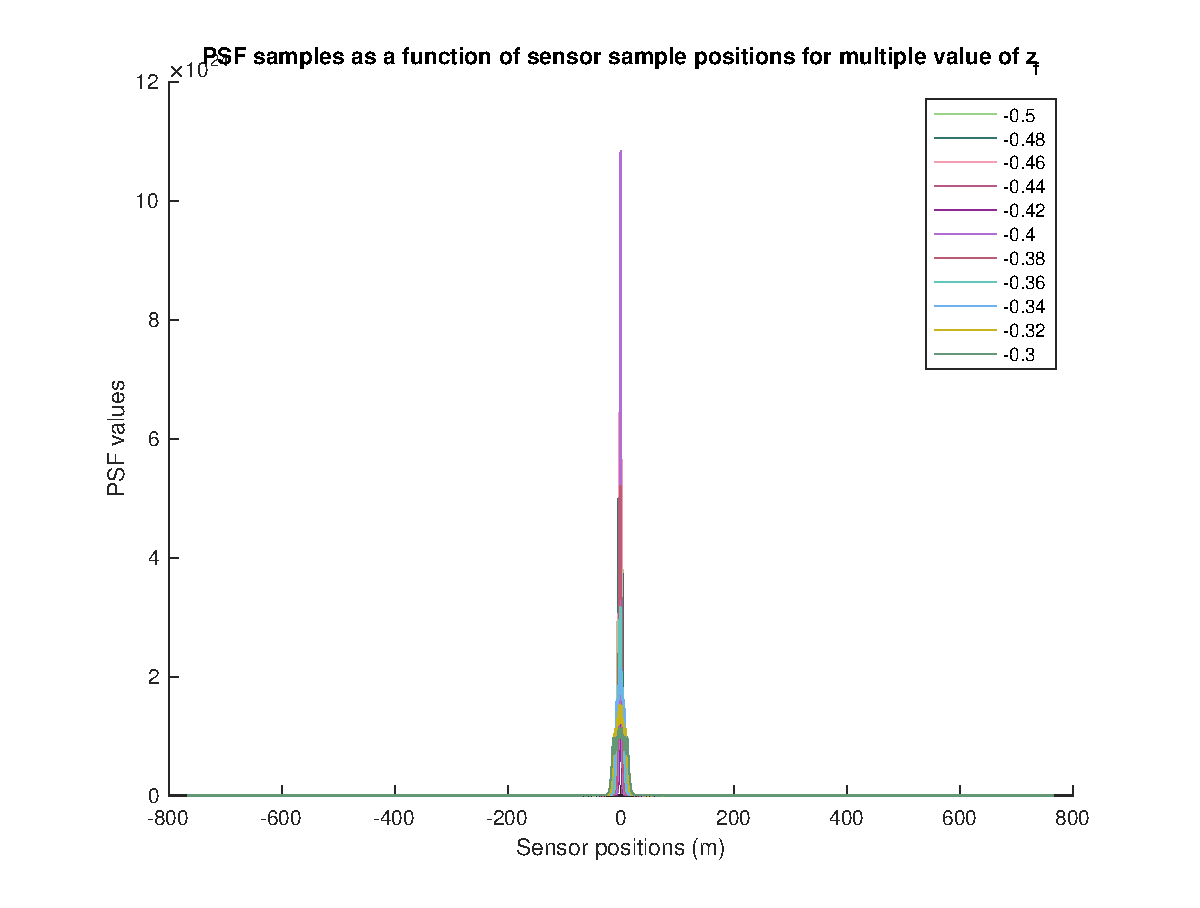
\includegraphics[width=\columnwidth]{img/psf_multiple_fresnel.eps}
  \caption{PSF results of the simulation with Fresnel synthesis, with multiple $z_f$ values between $-0.5$ and $-0.3$}
\end{figure}

\begin{figure}
  \label{fig:psf_multiple_rs}
  \centering
  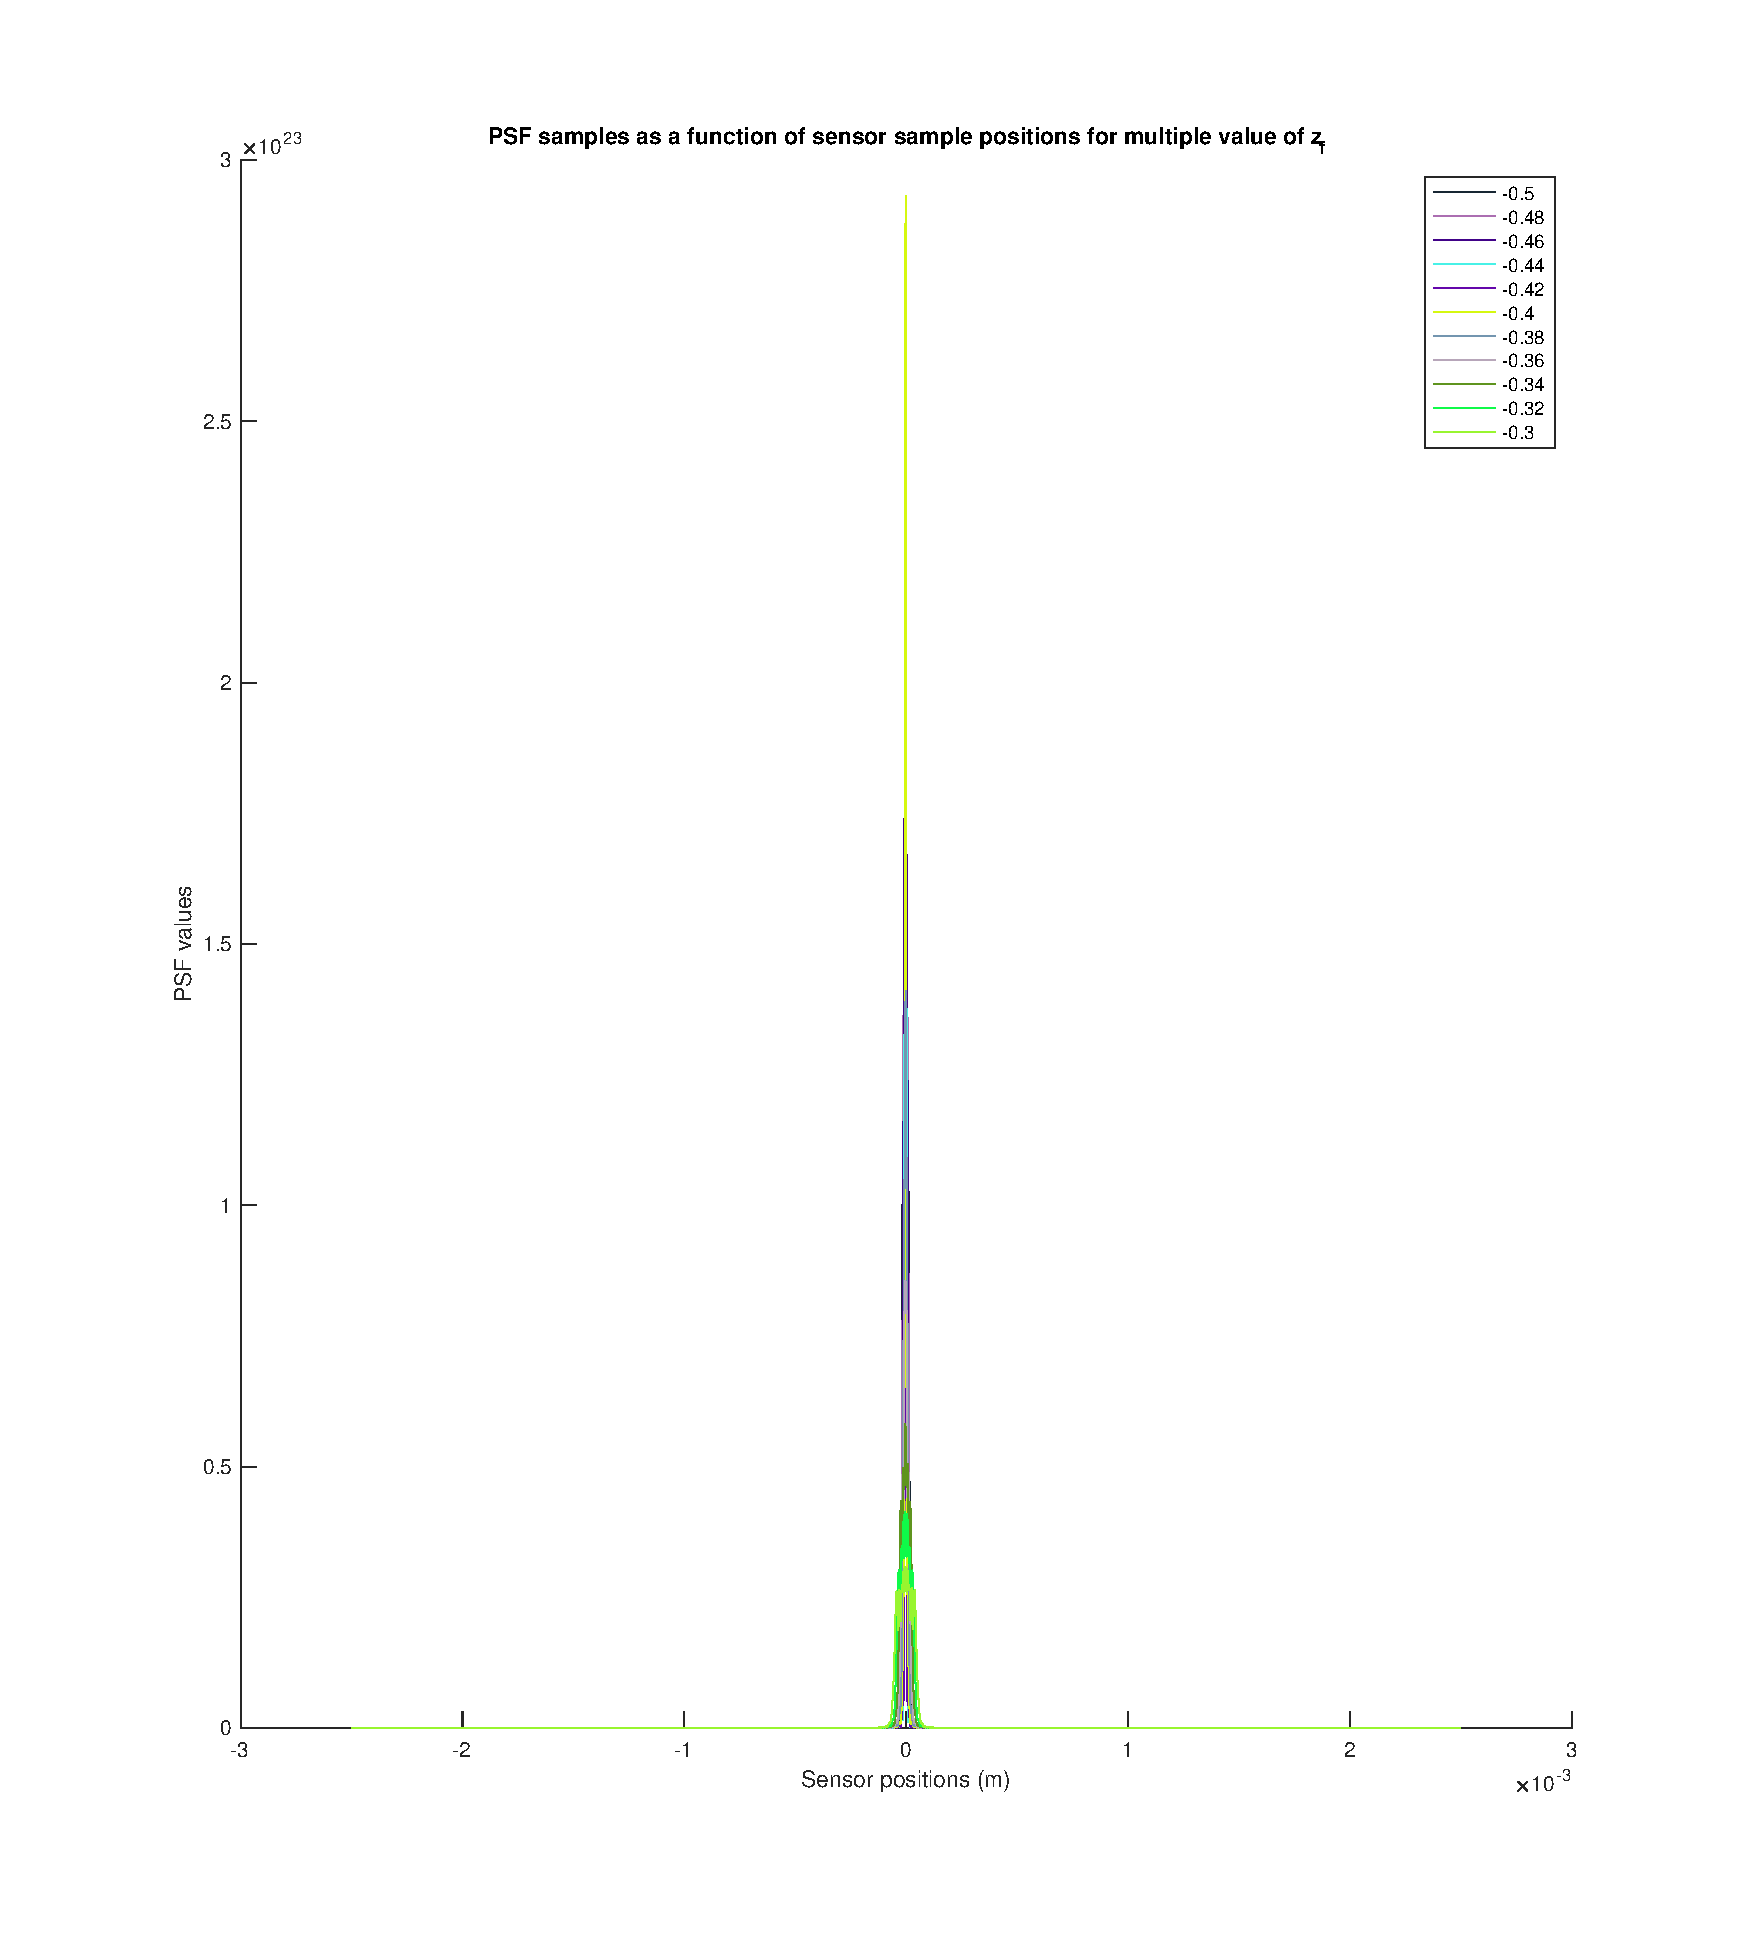
\includegraphics[width=\columnwidth]{img/psf_multiple_rs.eps}
  \caption{PSF results of the simulation with Rayleigh-Sommerfield synthesis, with multiple $z_f$ values between $-0.5$ and $-0.3$}
\end{figure}

\begin{figure}
  \label{fig:psf_multiple_hs}
  \centering
  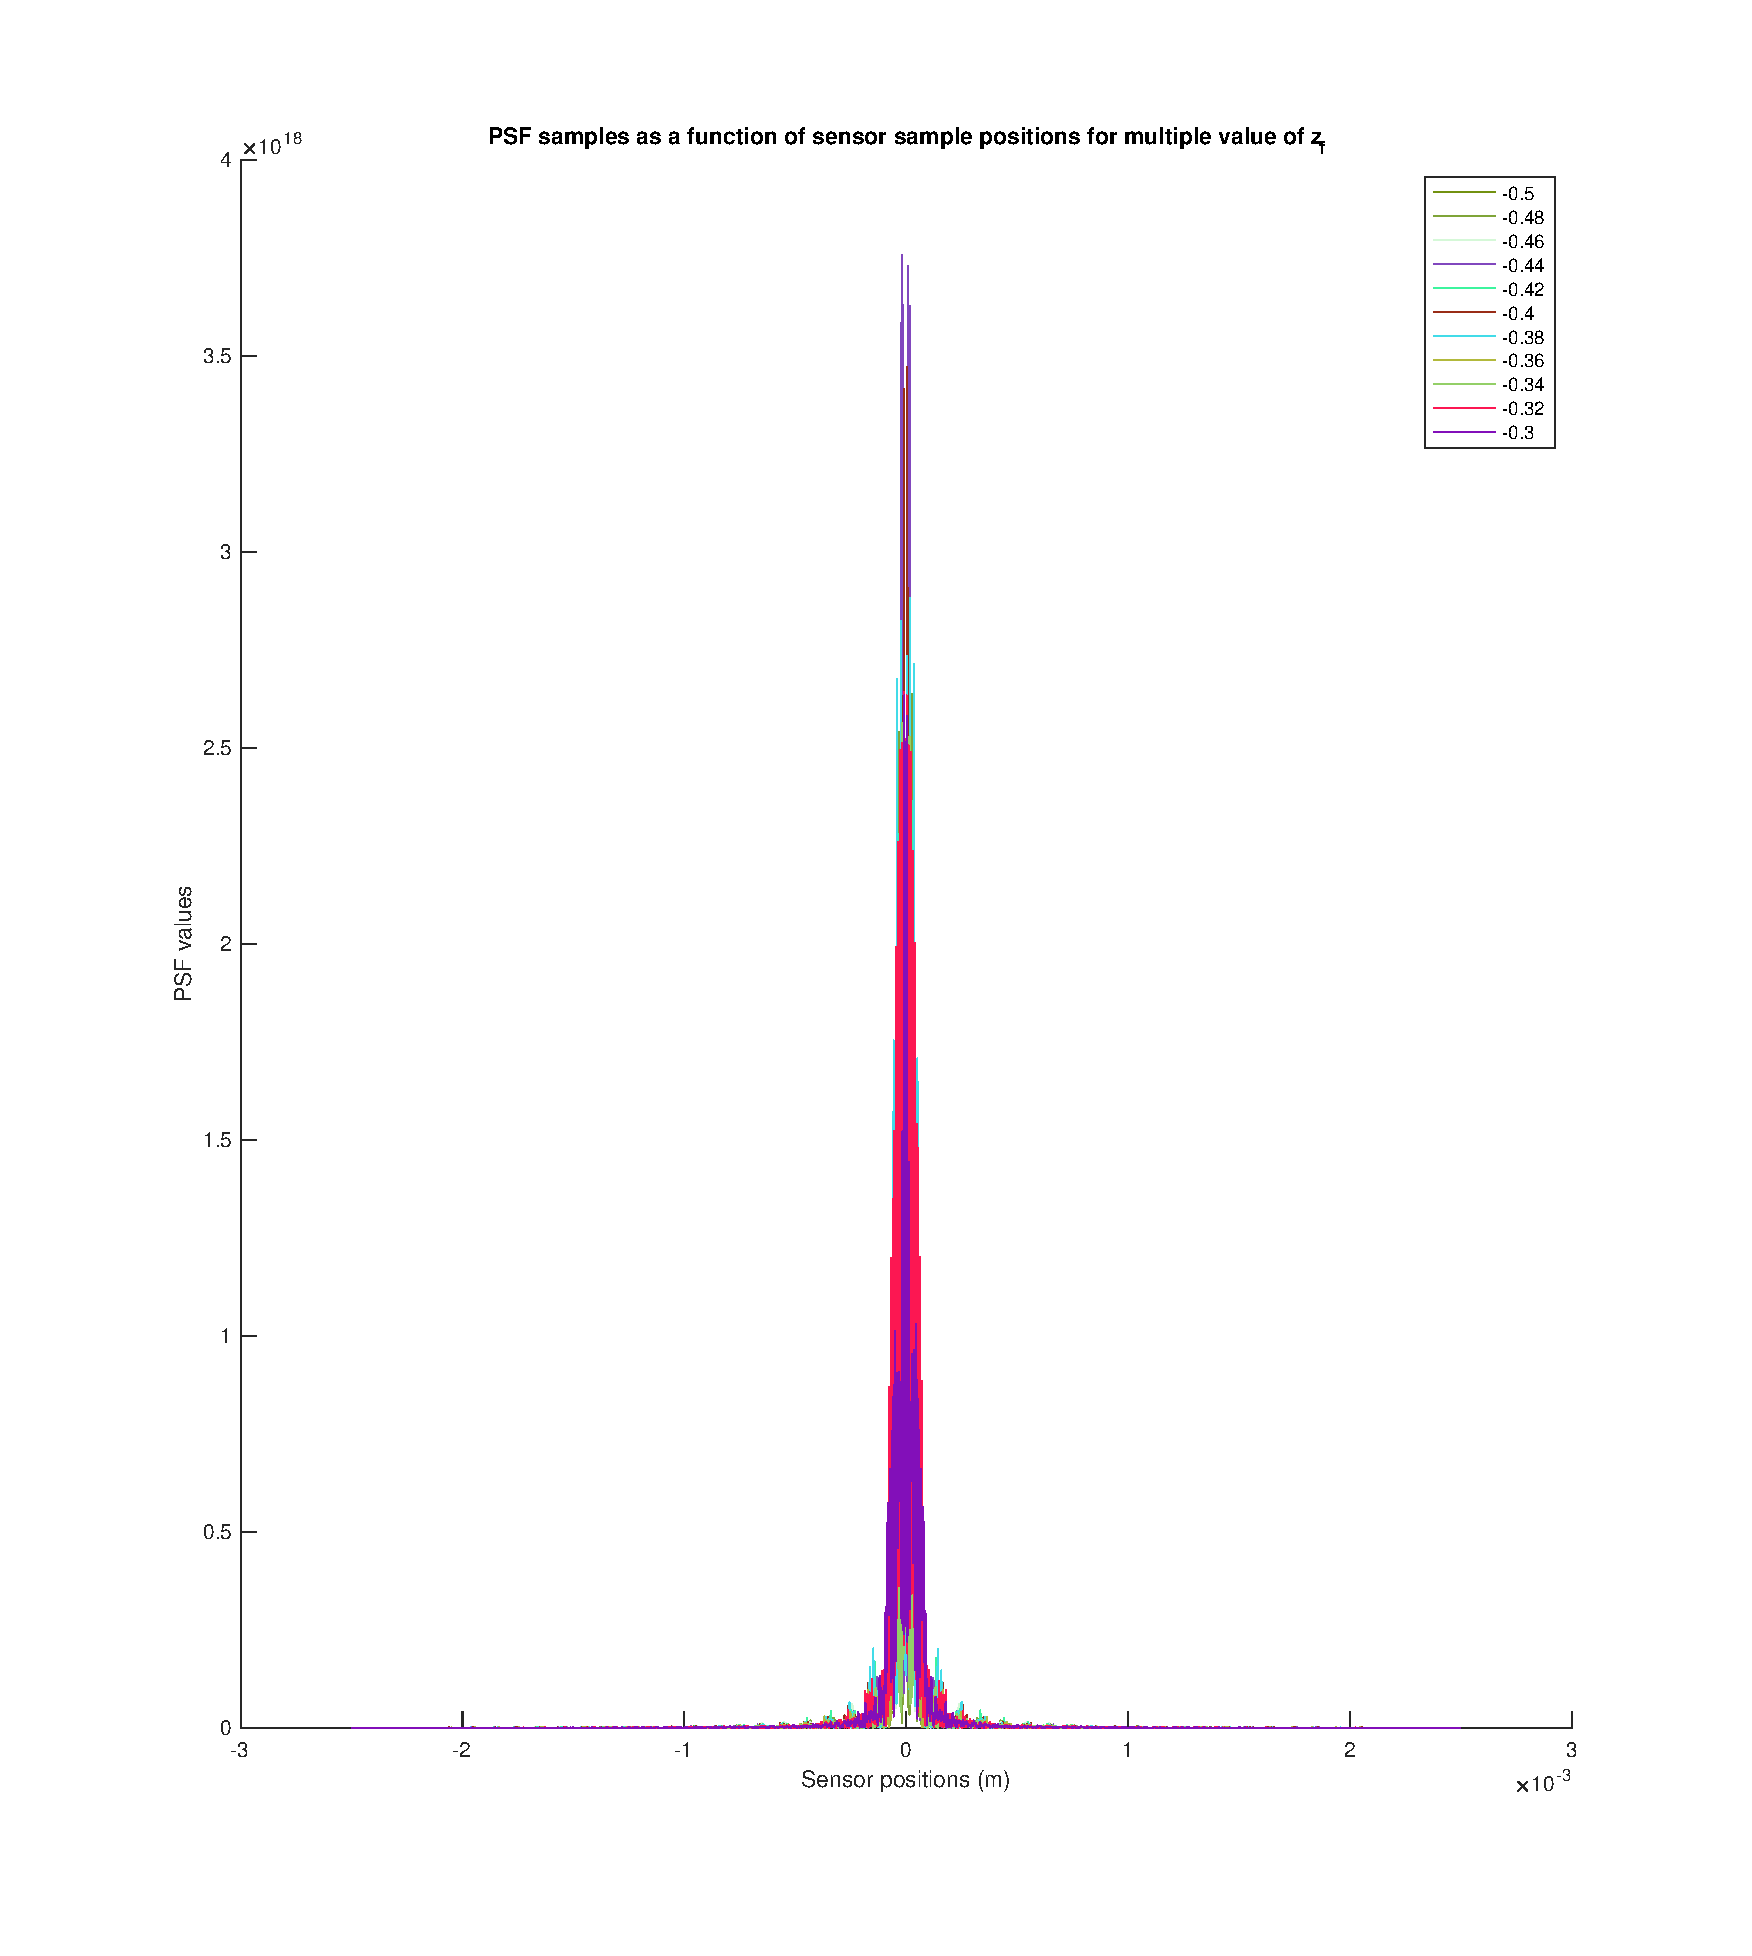
\includegraphics[width=\columnwidth]{img/psf_multiple_hs.eps}
  \caption{PSF results of the simulation with holograpic stereograph synthesis, with multiple $z_f$ values between $-0.5$ and $-0.3$}
\end{figure}


\section{MTF Analysis}
With the multiple PSF images we performed MTF analysis to obtain the value of $z_f$ which would provide the sharpest image

\begin{figure}
  \label{fig:mtf_fresnel}
  \centering
  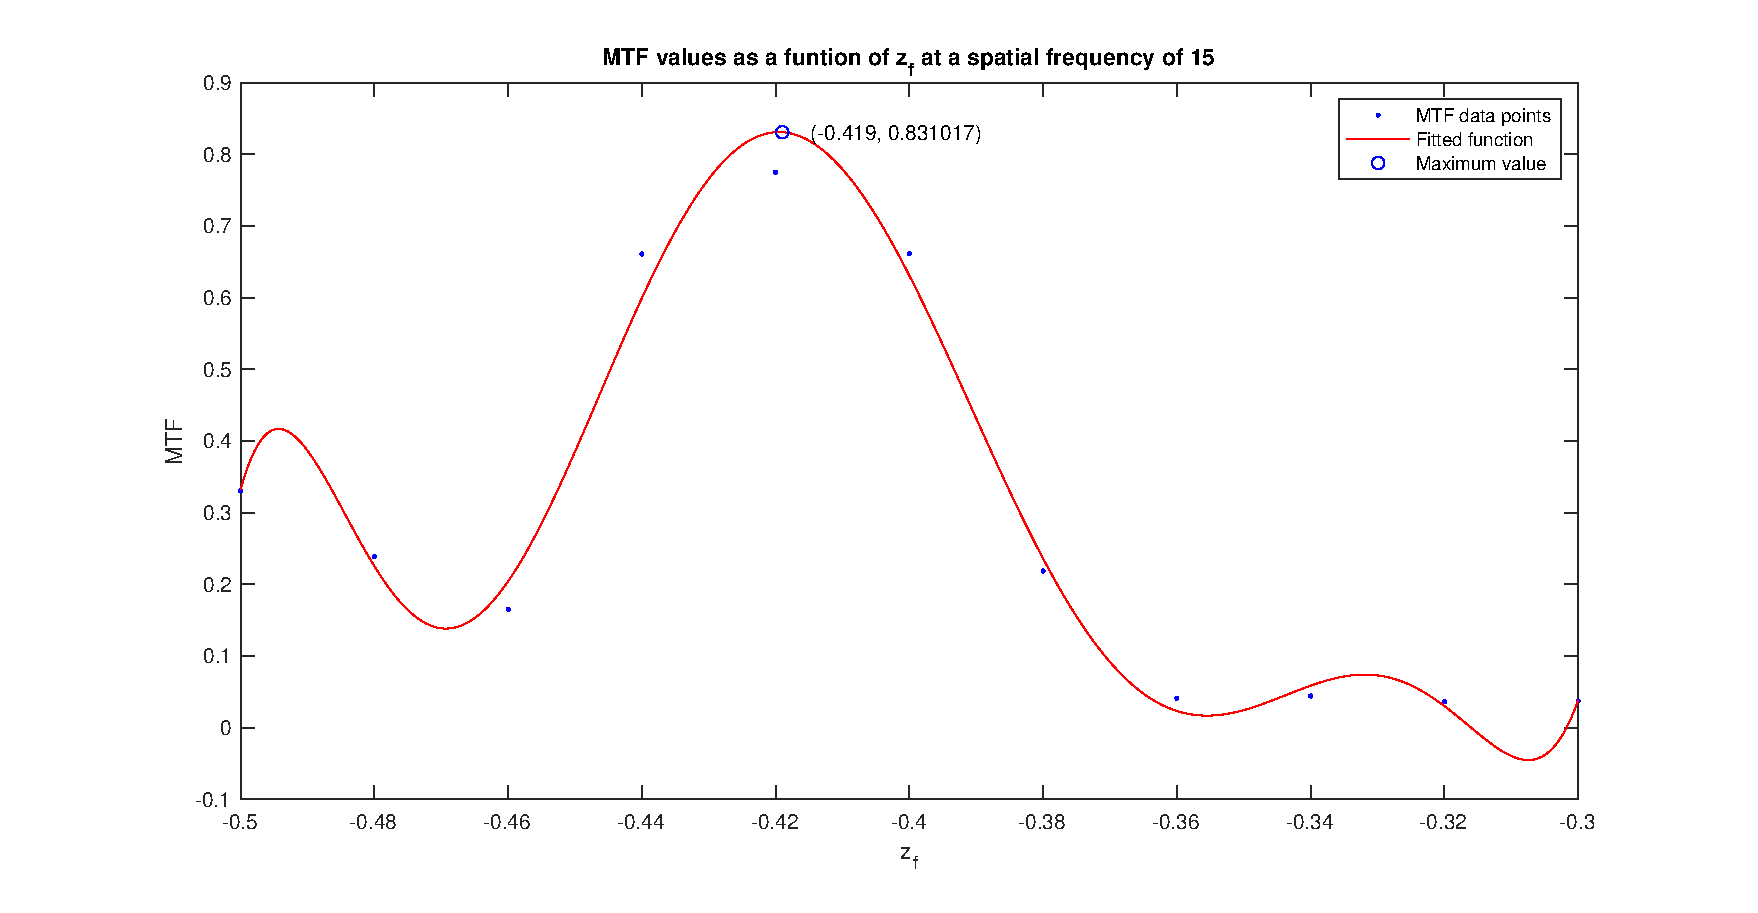
\includegraphics[width=\columnwidth]{img/mtf_fresnel.eps}
  \caption{MTF analysis results for Fresnel synthesis}
\end{figure}

\begin{figure}
  \label{fig:mtf_rs}
  \centering
  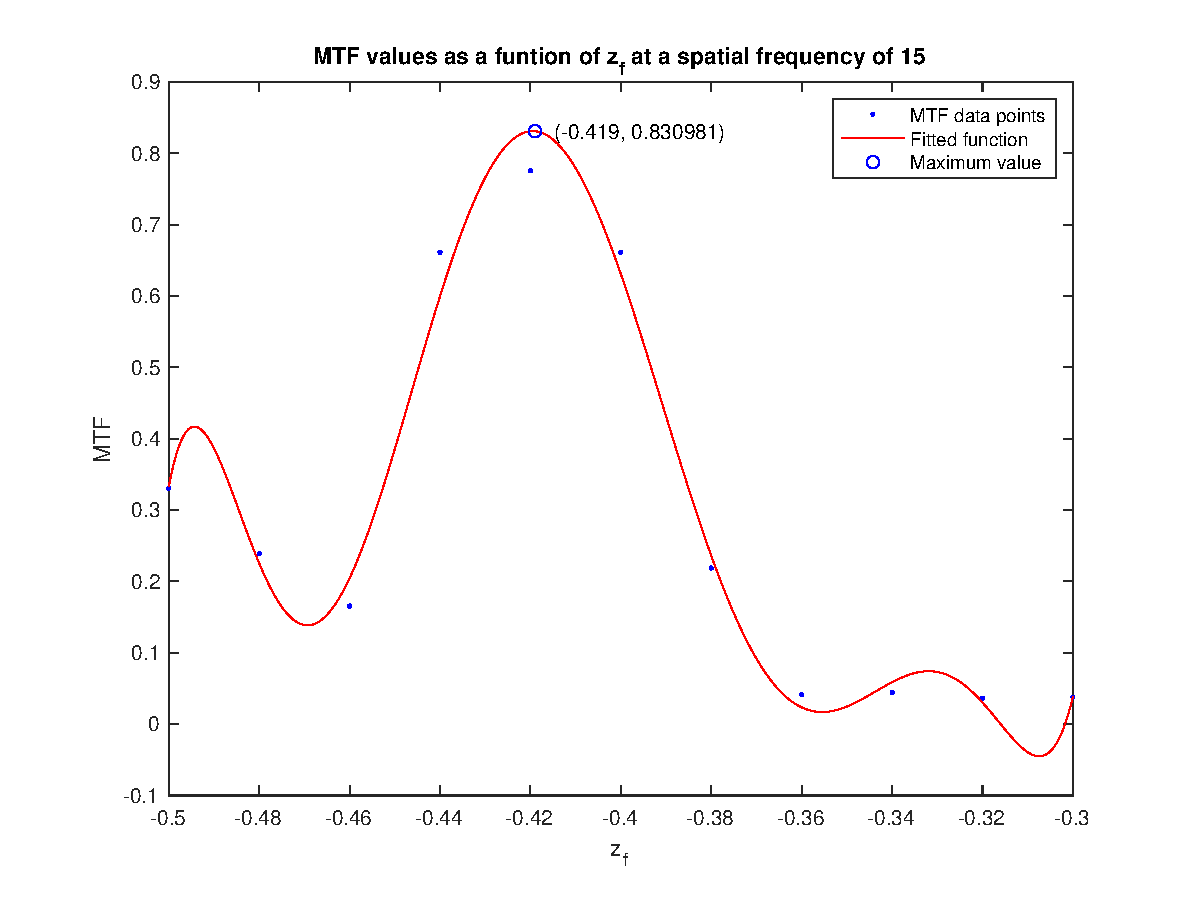
\includegraphics[width=\columnwidth]{img/mtf_rs.eps}
  \caption{MTF analysis results for Rayleigh-Sommerfield synthesis}
\end{figure}

\begin{figure}
  \label{fig:mtf_hs}
  \centering
  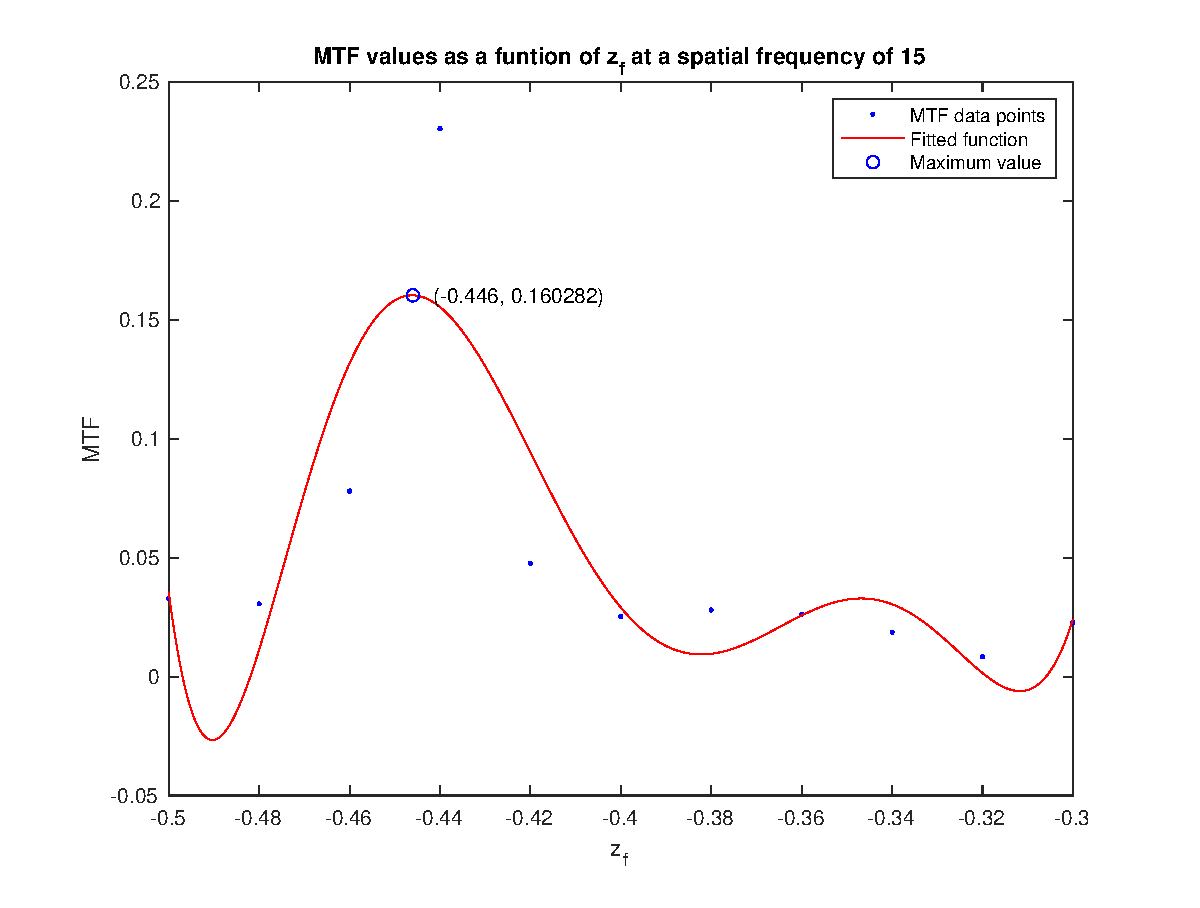
\includegraphics[width=\columnwidth]{img/mtf_hs.eps}
  \caption{MTF analysis results for Holographic stereograph synthesis}
\end{figure}


\chapter{Conclusions}

\label{ch:conclusions}


%
% The bibliography, i.e the list of references
%
\newpage

\printbibliography[title=References]
\addcontentsline{toc}{chapter}{References}

\appendix
\pagestyle{headings}



%
% a) Not-so-handy way, but at least it works
%
\def\appA{APPENDIX A. Something extra} % Define the name and numbering manually
\chapter*{\appA}                       % Create chapter heading
\markboth{\appA}{\appA}                % Set page header
\addcontentsline{toc}{chapter}{\appA}  % Include this in TOC
% Note that \label does not work with unnumbered chapter

Appendices are purely optional.  All appendices must be referred to in
the body text


\end{document}

